\documentclass{article}
\usepackage{polski}
\usepackage[utf8]{inputenc}
\usepackage[a4paper, total={7in, 10in}]{geometry}
\usepackage{listings}
\usepackage{amsmath}
\usepackage{subfig}
\usepackage{xcolor}
\usepackage{graphicx}
\usepackage[htt]{hyphenat}
\usepackage[colorlinks=true, allcolors=blue]{hyperref}

\definecolor{background}{rgb}{0.95,0.95,0.95}

\lstdefinestyle{mystyle}{
    backgroundcolor=\color{background},   
    keywordstyle=\color{purple},
    stringstyle=\color{orange},
    commentstyle=\color{brown},
    basicstyle=\ttfamily\footnotesize,
    breakatwhitespace=false,         
    breaklines=true,                 
    captionpos=b,                    
    keepspaces=true,                 
    numbers=left,                    
    numbersep=5pt,                  
    showspaces=false,                
    showstringspaces=false,
    showtabs=false,                  
    tabsize=2
}

\lstset{style=mystyle}

\title{Metody rozwiązywania układów równań liniowych}
\author{Michał Krause, 188592, Informatyka, sem. 4, gr. 4}
\date{08 maja 2023}

\begin{document}
\maketitle

\section{Wstęp}

Głównym celem projektu była implementacja w wybranym języku metod iteracyjnych i bezpośrednich rozwiązywania układów równań liniowych oraz ich analiza.

Analizowanymi metodami były metody iteracyjne Jacobiego oraz Gaussa-Seidla i metoda bezpośrednia faktoryzacji LU.

Do implementacji odpowiednich struktur oraz metod rozwiązywania układów równań liniowych został wykorzystany język Python.

\section{Metody rozwiązywania układów równań liniowych}

\subsection{Metody iteracyjne}

Iteracyjna metoda rozwiązywania równania macierzowego to metoda, która w kolejnych iteracjach wyznacza coraz dokładniej przybliżone rozwiązania równania macierzowego. Wykorzystując metody iteracyjne, przeważnie korzysta się z pewnych własności stopu, które zatrzymują program np. po osiągnięciu żądanej dokładności rozwiązania. Przeanalizowane zostały dwie metody iteracyjne: metoda Jacobiego i metoda Gaussa-Seidla.

\subsubsection{Metoda Jacobiego}

Realizację metody Jacobiego możemy przedstawić na dwa różne sposoby - w postaci operacji na pojedynczych elementach oraz w postaci macierzowej. Zakładając, że $x^{(k)}$ jest pewnym przybliżeniem dokładnego rozwiązania $x=A^{-1}b$, pierwszą z postaci można przedstawić w następujący sposób:

\[x_{i}^{(k+1)} = (b_{i} - \sum_{j=1}^{i-1} a_{ij}x_{j}^{(k)} - \sum_{j=i+1}^{n} a_{ij}x_{j}^{(k)}) / a_{ii}\]

W postaci macierzowej przyjmuje się, że macierz podzielona jest na trzy części: dolnotrójkątną $L$, górnotrójkątną $U$ oraz diagonalną $D$ ($A = -L - U + D$). W takim przypadku powyższy wzór możemy przedstawić w taki sposób:

\[x^{(k+1)} = D^{-1}(L+U)x^{(k)} + D^{-1}b\]

W powyższych schematach metody Jacobiego nie są uwzględnione aktualne wartości części elementów wektora $x$. Wykorzystywane są wartości z poprzednich iteracji pomimo tego, że dla części elementów znane są już nowo obliczone wartości.

\subsubsection{Metoda Gaussa-Seidla}

Jeżeli w powyższych wzorach uwzględnimy wartości obliczone w bieżącej iteracji, otrzymujemy schemat Gaussa-Seidla:

\[x_{i}^{(k+1)} = (b_{i} - \sum_{j=1}^{i-1} a_{ij}x_{j}^{(k+1)} - \sum_{j=i+1}^{n} a_{ij}x_{j}^{(k)}) / a_{ii}\]

\begin{center}oraz\end{center}

\[x^{(k+1)} = (D-L)^{-1}(Ux^{(k)}) + (D-L)^{-1}b\]

\subsection{Metody bezpośrednia}

Bezpośrednie metody rozwiązywania równania macierzowego to metody, które pozwalają wyznaczyć rozwiązanie równania macierzowego w skończonej liczbie operacji algebraicznych. W metodach bezpośrednich liczba wymaganych operacji algebraicznych silnie wzrasta wraz ze wzrostem rozmiaru macierzy, jednak umożliwiają one wyznaczenie rozwiązania z dużą dokładnością.

\subsubsection{Metoda faktoryzacji LU}

Metoda faktoryzacji LU jest wariantem metody eliminacji Gaussa. Polega na rozkładzie współczynników macierzy na iloczyn dwóch macierzy trójkątnych: dolnotrójkątnej $L$ i górnotrójkątnej $U$ (inne niż w przypadku metod iteracyjnych).

Aby rozwiązać układ równań $Ax=b$ należy stworzyć macierze $L$ i $U$ takie, że $LUx=b$, a następnie wektor pomocniczy $y=Ux$. Otrzymany wektor używamy w obliczeniu układu równań $Ly=b$ za pomocą podstawiania wprzód, a następnie w obliczeniu układu $Ux=y$, za pomocą podstawiania wstecz.

\section{Implementacja metod rozwiązywania układów równań}

\subsection{Struktura macierzy oraz metody pomocnicze}

Aby zrealizować projekt, została stworzona struktura macierzy, opierająca się na listach w Pythonie. Struktura ta zawiera dwuwymiarową tablicę oraz pomocnicze ilości kolumn i rzędów. Zdefiniowano własne operatory operacji arytmetycznych, m. in. dodawania, mnożenia i negacji.

\vspace{0.75em}
\begin{lstlisting}[language=Python, caption=Definicja klasy \texttt{matrix}]
class matrix:
    def __init__(self, row=0, col=0, mat=None):
        if mat is None:
            self.matrix = [[0 for _ in range(col)] for _ in range(row)]
            self.row = row
            self.col = col
        else:
            self.matrix = mat
            self.row = len(mat)
            self.col = len(mat[0])

    def __str__(self):
        s = ""
        for i in range(self.row):
            s += self.matrix[i].__str__() + "\n"
        return s

    def __add__(self, other):
        result = matrix(self.row, self.col)
        for i in range(self.row):
            for j in range(self.col):
                result.matrix[i][j] = self.matrix[i][j] + other.matrix[i][j]
        return result

    def __neg__(self):
        result = matrix(self.row, self.col)
        for i in range(self.row):
            for j in range(self.col):
                result.matrix[i][j] = -self.matrix[i][j]
        return result

    def __sub__(self, other):
        return self + (-other)

    def __mul__(self, other):
        result = matrix(self.row, other.col)
        for i in range(self.row):
            for j in range(other.col):
                for k in range(self.col):
                    result.matrix[i][j] += self.matrix[i][k] * other.matrix[k][j]
        return result
\end{lstlisting}
\newpage

Do metody bezpośredniej faktoryzacji LU zaimplementowanej w zadaniu wykorzystano metody podstawienia wprzód i wstecz oraz faktoryzacji:

\vspace{0.75em}
\begin{lstlisting}[language=Python, caption=Implementacja metod podstawienia wprzód/wstecz oraz faktoryzacji]
def lu_factorization(A):
    L = matrix(A.row, A.col)
    U = matrix(A.row, A.col)
    for i in range(A.row):
        for j in range(A.col):
            if i == j:
                L.matrix[i][j] = 1
            U.matrix[i][j] = A.matrix[i][j]
    for k in range(A.row - 1):
        for j in range(k + 1, A.row):
            L.matrix[j][k] = U.matrix[j][k] / U.matrix[k][k]
            for i in range(k, A.row):
                U.matrix[j][i] -= L.matrix[j][k] * U.matrix[k][i]
    return L, U


def forward_substitution(L, b):
    x = matrix(b.row, 1)
    for i in range(b.row):
        x.matrix[i][0] = b.matrix[i][0]
        for j in range(i):
            x.matrix[i][0] -= L.matrix[i][j] * x.matrix[j][0]
        x.matrix[i][0] /= L.matrix[i][i]
    return x


def backward_substitution(U, b):
    x = matrix(b.row, 1)
    for i in range(b.row - 1, -1, -1):
        x.matrix[i][0] = b.matrix[i][0]
        for j in range(i + 1, b.row):
            x.matrix[i][0] -= U.matrix[i][j] * x.matrix[j][0]
        x.matrix[i][0] /= U.matrix[i][i]
    return x
\end{lstlisting}
\vspace{1.5em}

W celu określenia punktu, w którym algorytmy iteracyjne zatrzymywały wyznaczanie rozwiązania została wykorzystana norma euklidesowa wektora residuum. Po przekroczeniu przez nią pewnego progu algorytmy zatrzymują pracę.

\vspace{0.75em}
\begin{lstlisting}[language=Python, caption=Definicja metod wyznaczania normy i residuum]
def residual(A, x, b):
    res = matrix(b.row, 1)
    for i in range(b.row):
        res.matrix[i][0] = -b.matrix[i][0]
        for j in range(b.row):
            res.matrix[i][0] += A.matrix[i][j] * x.matrix[j][0]
    return res


def norm(x):
    n = 0
    for i in range(x.row):
        n += x.matrix[i][0] ** 2
    return n ** 0.5
\end{lstlisting}

\newpage

\subsection{Metody rozwiązania układów równań}

Implementacja metod iteracyjnych (Jacobiego i Gaussa-Seidla) została zrealizowana za pomocą schematów działających na pojedynczych elementach:

\vspace{0.5em}
\begin{lstlisting}[language=Python, caption=Implementacja metody Jacobiego]
def solve_jacobi(A, b, x0, epsilon):
    x = matrix(x0.row, 1)
    iterations = 0
    upper_bound = 1e10
    norm_res_list = []
    for i in range(x.row):
        x.matrix[i][0] = x0.matrix[i][0]
    while True:
        x1 = matrix(x.row, 1)
        for i in range(x.row):
            x1.matrix[i][0] = b.matrix[i][0]
            for j in range(x.row):
                if j != i:
                    x1.matrix[i][0] -= A.matrix[i][j] * x.matrix[j][0]
            x1.matrix[i][0] /= A.matrix[i][i]
        iterations += 1
        norm_res = norm(residual(A, x1, b))
        norm_res_list.append(norm_res)
        if norm_res < epsilon:
            break
        if norm_res > upper_bound:
            print("Jacobi method does not converge, stopping")
            break
        for i in range(x.row):
            x.matrix[i][0] = x1.matrix[i][0]
    return x1, iterations, norm_res_list
\end{lstlisting}
\begin{lstlisting}[language=Python, caption=Implementacja metody Gaussa-Seidla]
def solve_gauss_seidl(A, b, x0, epsilon):
    x = matrix(x0.row, 1)
    iterations = 0
    upper_bound = 1e10
    norm_res_list = []
    for i in range(x.row):
        x.matrix[i][0] = x0.matrix[i][0]
    while True:
        x1 = matrix(x.row, 1)
        for i in range(x.row):
            x1.matrix[i][0] = b.matrix[i][0]
            for j in range(x.row):
                if j != i:
                    if j < i:
                        x1.matrix[i][0] -= A.matrix[i][j] * x1.matrix[j][0]
                    else:
                        x1.matrix[i][0] -= A.matrix[i][j] * x.matrix[j][0]
            x1.matrix[i][0] /= A.matrix[i][i]
        iterations += 1
        norm_res = norm(residual(A, x1, b))
        norm_res_list.append(norm_res)
        if norm_res < epsilon:
            break
        if norm_res > upper_bound:
            print("Gauss-Seidl method does not converge, stopping")
            break
        for i in range(x.row):
            x.matrix[i][0] = x1.matrix[i][0]
    return x1, iterations, norm_res_list
\end{lstlisting}
\vspace{1.25em}

Metoda faktoryzacji LU została zaimplementowana w następujący sposób:

\vspace{0.75em}
\begin{lstlisting}[language=Python, caption=Implementacja metody faktoryzacji LU]
def solve_lu_factorization(A, b):
    L, U = lu_factorization(A)
    y = forward_substitution(L, b)
    x = backward_substitution(U, y)
    return x, norm(residual(A, x, b))
\end{lstlisting}

\newpage

\section{Analiza działania metod rozwiązywania układów równań liniowych}

\subsection{Porównanie metod Jacobiego i Gaussa-Seidla}

Do porównania ilości iteracji wymaganej do uzyskania wyniku o określonej wielkości normy residuum ($10^{-9}$) rozwiązywano układ $Ax=b$. Zdefiniowano macierz pasmową $A$, gdzie główna diagonala zawierała elementy $a1=10$, dwie sąsiednie oraz dwie skrajne z elementami $a2=a3=-1$. Macierz ta miała rozmiar $N\times N$, gdzie $N=992$. Wektor $b$ o długości $N$ przyjął wartości $sin(9*n)$, gdzie $n$ jest $n$-tym elementem wektora. W stanie początkowym (przed pierwszą iteracją) wektor $x$ przyjął wartości $x_i=1$.

Dla takich danych, metoda Jacobiego do osiągnięcia określonej normy residuum potrzebowała \textbf{29} iteracji, a metoda Gaussa-Seidla jedynie \textbf{19}. Dobrze pokazuje to, że schemat Gaussa-Seidla lepiej sobie radzi niż metoda Jacobiego. Dzieje się tak, ponieważ metoda Gaussa-Seidla działa na wynikach policzonych w bieżącej iteracji, a nie w poprzedniej, tak jak schemat Jacobiego.

Gdy przyjęto takie same dane jak w poprzednim teście, z wyjątkiem $a1=3$, metody iteracyjne nie zbiegały się. Oznacza to, że norma z błędu rezydualnego rosła do nieskończoności, zamiast maleć do zera. Zjawisko to zachodzi, ponieważ macierz $A$ dla nowej wartości $a1$ nie jest diagonalnie dominująca, co oznacza, że wartości bezwzględne elementów na głównej przekątnej są mniejsze bądź równe sumy wartości bezwzględnych pozostałych elementów. Łatwo można to zauważyć, gdyż w każdym wierszu poza dwoma pierwszymi i ostatnimi, wartość elementu należącego do przekątnej wynosi $3$, pozostałych elementów wiersza $-1$, a $|3| < |-4|$.

Poniżej znajdują się wykresy, które pokazują zbieżność i rozbieżność metod iteracyjnych w podanych przypadkach:

\begin{figure}[h!]%
    \centering
    \subfloat[\centering Jacobi, $a1=10$]{{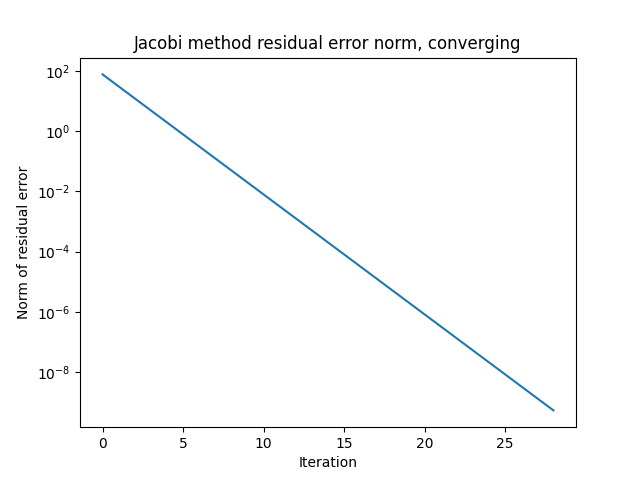
\includegraphics[width=8cm]{img/jacobi_con.png} }}%
    \qquad
    \subfloat[\centering Gauss-Seidl, $a1=10$]{{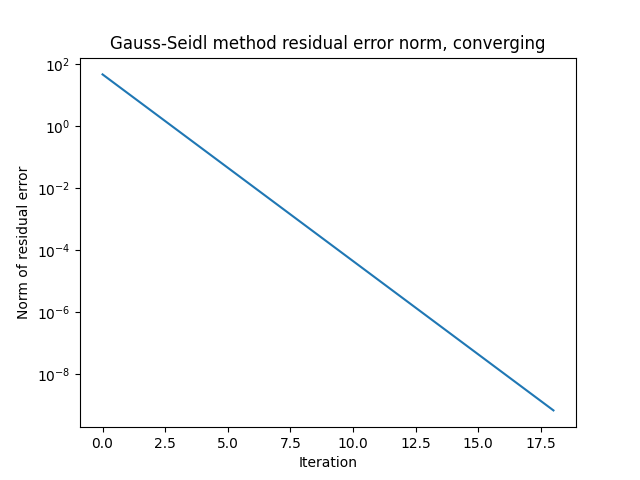
\includegraphics[width=8cm]{img/gauss_con.png} }}%
    \caption{Zbieżność dla $a1=10$}%
    \label{fig:example}%
\end{figure}

\begin{figure}[h!]%
    \centering
    \subfloat[\centering Jacobi, $a1=3$]{{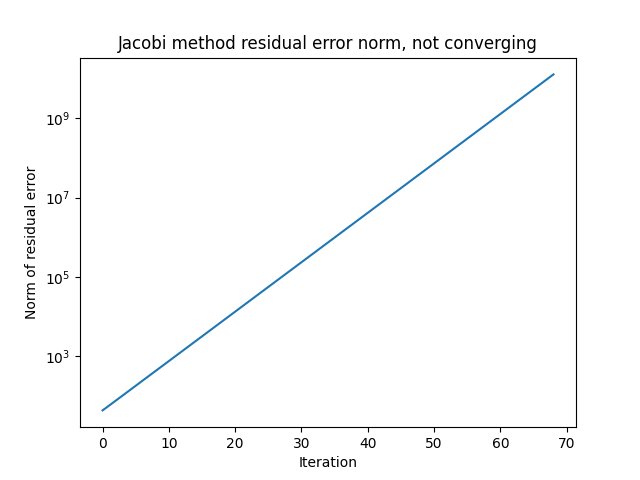
\includegraphics[width=8cm]{img/jacobi_ncon.png} }}%
    \qquad
    \subfloat[\centering Gauss-Seidl, $a1=3$]{{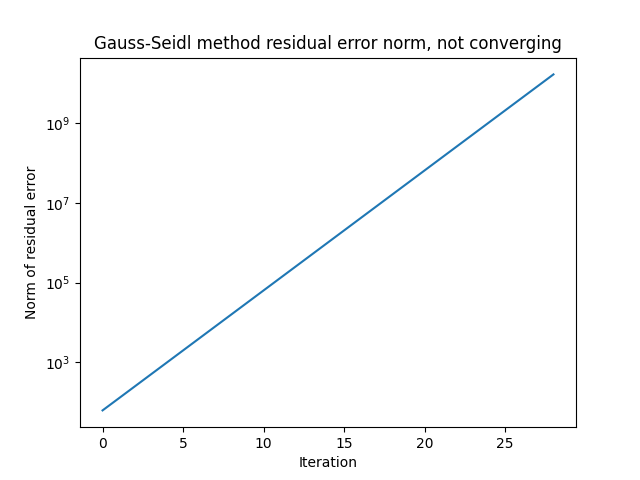
\includegraphics[width=8cm]{img/gauss_ncon.png} }}%
    \caption{Brak zbieżności dla $a1=3$}%
    \label{fig:example}%
\end{figure}

\subsection{Analiza wyniku metody bezpośredniej}

Dla układu równań z poprzedniego testu ($a1=3$, $a2=a3=-1$, b takie samo) uruchomiono metodę faktoryzacji LU. Wynik, jaki osiągnęła, charakteryzował się normą z residuum wynoszącą około $2.52026*10^{-13}$. Oznacza to, że wynik jest bardzo dokładny, co jest charakterystyczne dla metod bezpośrednich. Kosztem takiej dokładności tej metody jest długi czas wykonywania.

\subsection{Porównanie czasu wykonywania metod w zależności od rozmiaru macierzy}

Ostatnim testem było porównanie czasu wykonywania metod w zależności od wielkości wartości $N$. Dane przyjęły wartości z pierwszego testu, czyli $a1=10$, $a2=a3=-1$, $b_n=sin(9*n)$, gdzie $n$ to $n$-ty element wektora b. Macierz $A$ została stworzona w ten sam sposób co w poprzednich testach, czyli jest macierzą pasmową. Przeprowadzonych zostało 6 testów, dla $N=[100, 200, 500, 1000, 2000, 3000]$. Po wyznaczeniu czasu wykonywania w zależności od $N$ i przełożeniu go na wykresy, otrzymano takie wyniki:

\begin{figure}[h!]
  \centering
  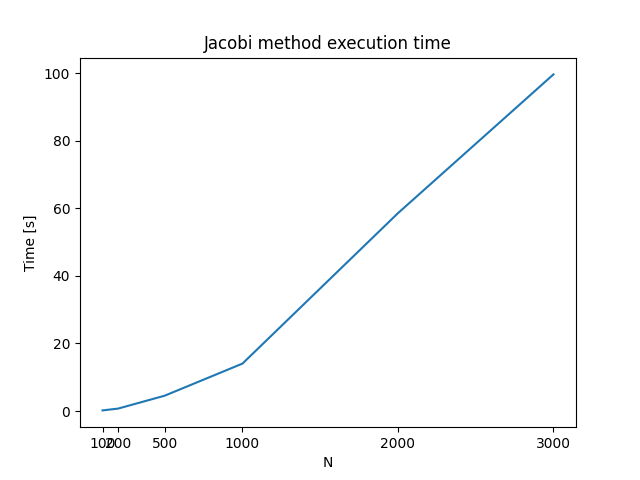
\includegraphics[width=0.6\textwidth]{img/jacobi.png}
  \caption{Wykres zależności czasu od N dla metody Jacobiego}
\end{figure}

\begin{figure}[h!]
  \centering
  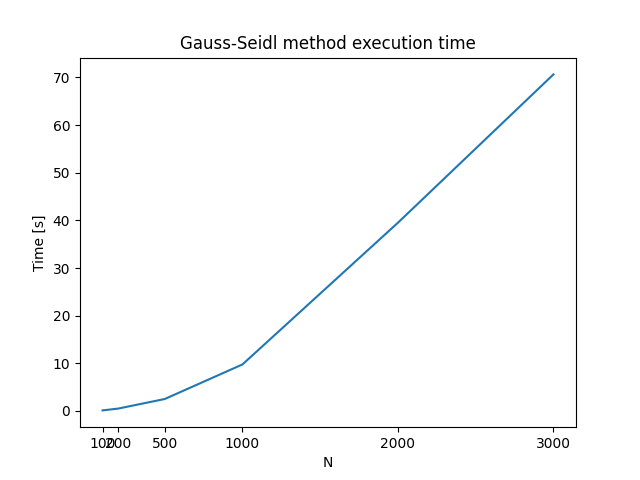
\includegraphics[width=0.6\textwidth]{img/gauss.png}
  \caption{Wykres zależności czasu od N dla metody Jacobiego}
\end{figure}

\begin{figure}[h!]
  \centering
  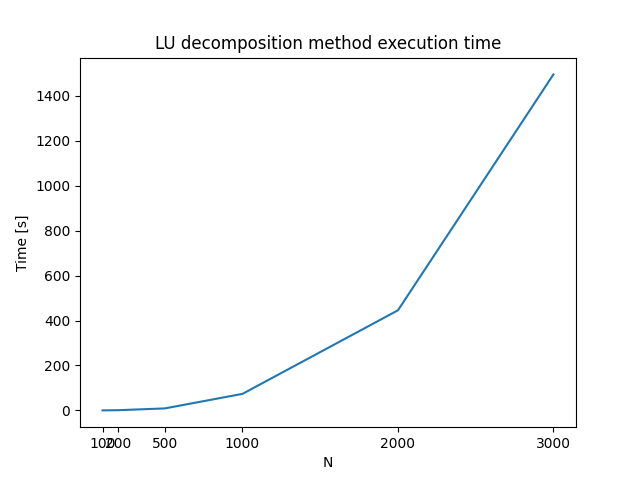
\includegraphics[width=0.6\textwidth]{img/lu.png}
  \caption{Wykres zależności czasu od N dla metody faktoryzacji LU}
\end{figure}

Z wykresów wynika, że czas wykonywania obydwóch metod iteracyjnych rośnie w takim samym tempie w zależności od wielkości $N$, aczkolwiek jak już wcześniej wspomniano, metoda Gaussa-Seidla działa szybciej niż metoda Jacobiego.

Metoda faktoryzacji LU rośnie w większym tempie niż badane metody iteracyjne. Dla małych wartości $N$ czas wykonywania był podobny, lecz bardzo szybko przewyższył czas wykonywania metod iteracyjnych. Dla $N=3000$ metody iteracyjne wykonują się mniej więcej półtorej minuty, a metoda bezpośrednia około dwadzieścia pięć minut.

\section{Wnioski}

Metody iteracyjne, w porównaniu do metod bezpośrednich, dążą do wyniku krok po kroku, uzyskując coraz dokładniejszy wynik. Z drugiej strony, metody bezpośrednie uzyskują w skończonej ilości operacji wynik, który cechuje się wysoką dokładnością. 

Zaletą metod iteracyjnych jest ich szybkość, gdyż ich tempo wzrostu jest mniejsze niż metod bezpośrednich. Jest to szczególnie zauważalne porównując wykresy zależności czasu od wielkości $N$, gdyż w ostatnich przypadkach czas ten przekraczał czas metod iteracyjnych kilkunastokrotnie. 

Użycie metod iteracyjnych wymaga spełnienia odpowiednich warunków przez macierze, co jest widoczne w jednym z badanych przypadków, gdy algorytmy nie zbiegały się one do poprawnego wyniku.

\end{document}